% !TEX TS-program = pdflatex
% !TEX encoding = UTF-8 Unicode

% This is a simple template for a LaTeX document using the "article" class.
% See "book", "report", "letter" for other types of document.

\documentclass[11pt]{article} % use larger type; default would be 10pt

\usepackage[utf8]{inputenc} % set input encoding (not needed with XeLaTeX)
\usepackage{amsmath,amsthm, amssymb}

%%% Examples of Article customizations
% These packages are optional, depending whether you want the features they provide.
% See the LaTeX Companion or other references for full information.

%%% PAGE DIMENSIONS
\usepackage[margin=0.6in]{geometry} % to change the page dimensions
\geometry{a4paper} % or letterpaper (US) or a5paper or....
% \geometry{margin=2in} % for example, change the margins to 2 inches all round
% \geometry{landscape} % set up the page for landscape
%   read geometry.pdf for detailed page layout information

\usepackage{graphicx} % support the \includegraphics command and options
\usepackage[makeroom]{cancel}
\renewcommand{\familydefault}{\sfdefault}
% \usepackage[parfill]{parskip} % Activate to begin paragraphs with an empty line rather than an indent

%%% PACKAGES
\usepackage{booktabs} % for much better looking tables
\usepackage{array} % for better arrays (eg matrices) in maths
\usepackage{paralist} % very flexible & customisable lists (eg. enumerate/itemize, etc.)
\usepackage{verbatim} % adds environment for commenting out blocks of text & for better verbatim
\usepackage{subfig} % make it possible to include more than one captioned figure/table in a single float
% These packages are all incorporated in the memoir class to one degree or another...

%%% HEADERS & FOOTERS
\usepackage{fancyhdr} % This should be set AFTER setting up the page geometry
\pagestyle{fancy} % options: empty , plain , fancy
\renewcommand{\headrulewidth}{0pt} % customise the layout...
\lhead{}\chead{}\rhead{}
\lfoot{}\cfoot{\thepage}\rfoot{}

%%% SECTION TITLE APPEARANCE
\usepackage{sectsty}
\allsectionsfont{\sffamily\mdseries\upshape} % (See the fntguide.pdf for font help)
% (This matches ConTeXt defaults)

%%% ToC (table of contents) APPEARANCE
\usepackage[nottoc,notlof,notlot]{tocbibind} % Put the bibliography in the ToC
\usepackage[titles,subfigure]{tocloft} % Alter the style of the Table of Contents
\renewcommand{\cftsecfont}{\rmfamily\mdseries\upshape}
\renewcommand{\cftsecpagefont}{\rmfamily\mdseries\upshape} % No bold!

%%% END Article customizations

%%% The "real" document content comes below...

\title{Assignment-1, CMPSCI 688}
\author{Ashish Jain}
%\date{} % Activate to display a given date or no date (if empty),
         % otherwise the current date is printed 

\begin{document}
\maketitle

\section*{Question 1. Factorization}
{\raggedleft{}Joint distribution for any Bayesian Network is obtained as a product of these conditional distribution:}
\begin{align*}
P(X) = \prod_{i=1}^{N} P(X_i | Pa_{X_i}^{G}) \\
\end{align*}
Using the above equation, we can write the factorization for the given graph as follows:
\begin{align*}
P(A,G,BP,CH,HD,CP,EIA,ECG,HR) &= P(G).P(A).P(BP|G).P(CH|G, A).P(HD|BP, CH).P(HR|A, HD)\\
						      & P(CP|HD).P(EIA|HD).P(ECG|HD)
\end{align*}
\section*{Question 2. Likelihood Function}

Log likelihood function as an empirical average over the data set is given by following expression:

\begin{equation}
{\cal L}(\theta) = \dfrac{1}{N} \sum_{n=1}^{N} log P_{\theta}(x_{n}) \\
\end{equation}
\begin{equation}
P_{\theta}(X=x) = \prod_{d=1}^{D} P_{\theta}(X_{d} = x_{d}|X_{Pa(X_{d})} = x_{Pa(X_{d})}) \\
				= \prod_{d=1}^{D}\prod_{v=1}^{V}(\theta_{v|x_{Pa(X_{d})}}^{X_{d}})^{[x_{d}=v]}
\end{equation}
Using the above two equations we will write the probability expression for the given graph and than take log of it.
\begin{flalign*}
P_{\theta}(A,G,BP,CH,HD,CP,EIA,ECG,HR) &= P_{\theta}(A=a)P_{\theta}(G=g)P_{\theta}(BP=bp|G=g)\\
& P_{\theta}(CH=ch|G=g, A=a)P_{\theta}(HD=hd|BP=bp, CH=ch)\\
& P_{\theta}(HR=hr|A=a,HD=hd)P_{\theta}(CP=cp|HD=hd)\\
& P_{\theta}(EIA=eia|HD=hd)P_{\theta}(ECG=ecg|HD=hd) \\ \\
\end{flalign*}
\begin{flalign*}
{\cal L}(\theta) &= \dfrac{1}{N} \sum_{n=1}^{N} log P_{\theta}(x_{n}) \\ 
&= \dfrac{1}{N} \sum_{n=1}^{N} \sum_{g}[g_{n}=g]log P(G=g) + \dfrac{1}{N} \sum_{n=1}^{N} \sum_{a}[a_{n}=a]log P(A=a) \\
& + \dfrac{1}{N} \sum_{n=1}^{N} \sum_{bp,g}[bp_{n}=bp][g_{n}=g]log P(BP=bp|G=g) \\
& + \dfrac{1}{N} \sum_{n=1}^{N} \sum_{ch,a,g}[ch_{n}=ch][g_{n}=g][a_{n}=a]log P(CH=ch|G=g, A=a) \\
& + \dfrac{1}{N} \sum_{n=1}^{N} \sum_{hd,bp,ch}[hd_{n}=hd][bp_{n}=bp][ch_{n}=ch]log P(HD=hd|BP=bp,CH=ch) \\
& + \dfrac{1}{N} \sum_{n=1}^{N} \sum_{hr,a,hd}[hr_{n}=hr][a_{n}=a][hd_{n}=hd]log P(HR=hr|A=a,HD=hd) \\
& + \dfrac{1}{N} \sum_{n=1}^{N} \sum_{cp, hd}[cp_{n}=cp][hd_{n}=hd]log P(CP=cp|HD=hd) \\ 
& + \dfrac{1}{N} \sum_{n=1}^{N} \sum_{eia, hd}[eia_{n}=eia][hd_{n}=hd]log P(EIA=eia|HD=hd) \\
& + \dfrac{1}{N} \sum_{n=1}^{N} \sum_{ecg, hd}[ecg_{n}=ecg][hd_{n}=hd]log P(ECG=ecg|HD=hd) \\
\end{flalign*}

\begin{flalign*}
{\cal L}(\theta) &= \dfrac{1}{N} \sum_{n=1}^{N} \sum_{g}[g_{n}=g]log \theta_{a}^{A} + \dfrac{1}{N} \sum_{n=1}^{N} \sum_{a}[a_{n}=a]log \theta_{g}^{G} \\
& + \dfrac{1}{N} \sum_{n=1}^{N} \sum_{bp,g}[bp_{n}=bp][g_{n}=g]log \theta_{bp|g}^{BP} \\
& + \dfrac{1}{N} \sum_{n=1}^{N} \sum_{ch,a,g}[ch_{n}=ch][g_{n}=g][a_{n}=a]log \theta_{ch|g,a}^{CH} \\
& + \dfrac{1}{N} \sum_{n=1}^{N} \sum_{hd,bp,ch}[hd_{n}=hd][bp_{n}=bp][ch_{n}=ch]log \theta_{hd|ch,bp}^{HD} \\
& + \dfrac{1}{N} \sum_{n=1}^{N} \sum_{hr,a,hd}[hr_{n}=hr][a_{n}=a][hd_{n}=hd]log \theta_{hr|a,hd}^{HR} \\
& + \dfrac{1}{N} \sum_{n=1}^{N} \sum_{cp, hd}[cp_{n}=cp][hd_{n}=hd]log \theta_{cp|hd}^{CP} \\ 
& + \dfrac{1}{N} \sum_{n=1}^{N} \sum_{eia, hd}[eia_{n}=eia][hd_{n}=hd]log \theta_{eia|hd}^{EIA} \\
& + \dfrac{1}{N} \sum_{n=1}^{N} \sum_{ecg, hd}[ecg_{n}=ecg][hd_{n}=hd]log \theta_{ecg|hd}^{ECG} \\
\end{flalign*}
\section*{Question 4. Learning}
\begin{tabular}{|c|c|}
\hline
P(A)   & (A)   \\ \hline
0.1769 & \textless45   \\ \hline
0.3086 & 45-55 \\ \hline
0.5144 & \textgreater=55  \\ \hline
\end{tabular}
\vspace*{1em}\\
\begin{tabular}{|c|c|c|}
\hline
P(BP$|$G) & P(BP) & P(G)   \\ \hline
0.3658  & Low   & Female \\ \hline
0.6341  & High  & Female \\ \hline
0.472   & Low   & Male   \\ \hline
0.5279  & High  & Male   \\ \hline
\end{tabular}
\vspace*{1em}\\
\begin{tabular}{|c|c|c|c|}
\hline
P(HD$|$BP, CH) & HD & BP   & CH   \\ \hline
0.5263         & N  & Low  & Low  \\ \hline
0.4736         & Y  & Low  & Low  \\ \hline
0.5909         & N  & High & Low  \\ \hline
0.409          & Y  & High & Low  \\ \hline
0.5862         & N  & Low  & High \\ \hline
0.4137         & Y  & Low  & High \\ \hline
0.513          & N  & High & High \\ \hline
0.4869         & Y  & High & High \\ \hline
\end{tabular}
\vspace*{1em} \\ \\
\begin{tabular}{|c|c|c|c|}
\hline
P(HR$|$A, HD) & HR   & A      & HD \\ \hline
0.0606        & Low  & $<$45  & N  \\ \hline
0.9393        & High & $<$45  & N  \\ \hline
0.173         & Low  & 45-55 & N  \\ \hline
0.8269        & High & 45-55 & N  \\ \hline
0.3333        & Low  & $>=$55 & N  \\ \hline
0.6666        & High & $>=$55 & N  \\ \hline
0.6           & Low  & $<$45 & Y  \\ \hline
0.4           & High & $<$45 & Y  \\ \hline
0.5217        & Low  & 45-55 & Y  \\ \hline
0.4782        & High & 45-55 & Y  \\ \hline
0.5714        & Low  & $>=$55 & Y  \\ \hline
0.4285        & High & $>=$55 & Y  \\ \hline
\end{tabular}
\vspace*{1em}\\
\section*{5. Probability Queries}
We will use following joint probability expression for the given two queries:
\begin{align*}
P(A,B) &= P(A|B).P(B)
\end{align*}
\subsection*{(a)}
Random variable CH (cholestrol) can take following two values: Low and High. Let us solve the query using $CH=L$ using the above joint probability equation.
 \begin{flalign*}
  P(CH = L | A = 2, G = M, CP = None, BP = L, ECG = Normal, HR = L, EIA = No, HD = No) = \\
  \dfrac{P(CH = L, A = 2, G = M, CP = None, BP = L, ECG = Normal, HR = L, EIA = No, HD = No)}
          {P(A = 2, G = M, CP = None, BP = L, ECG = Normal, HR = L, EIA = No, HD = No)} =   \\ \\
   \dfrac{P(CH = L, A = 2, G = M, CP = None, BP = L, ECG = Normal, HR = L, EIA = No, HD = No) }
          {\sum_{ch \in (L, H) }P(CH = ch, A = 2, G = M, CP = None, BP = L, ECG = Normal, HR = L, EIA = No, HD = No)} = \tag{\text{marginalizing over CH} }\\ \\
   \dfrac{P(CH = L | A = 2, G = M)P(HD = L | CH = L, BP = L)}{\sum_{ch \in (L, H)} P(CH = ch | A = 2, G = M) P(HD = L| CH = ch, BP = L)} 
      = \tag{\text{Using factorization and conditional independence property, terms indepedent of CH will get cancelled out.} } \\
 \end{flalign*} \\
 By using learned CPT tables in Part 4 over training file 1, we get following answer for this Query: \\ \\
 {\small {
 $P(CH = L | A = 2, G = M, CP = None, BP = L, ECG = Normal, HR = L, EIA = No, HD = No) = $0.1522 }} \\
 {\small{
 $P(CH = H | A = 2, G = M, CP = None, BP = L, ECG = Normal, HR = L, EIA = No, HD = No) = $0.8477 }}  \\
\subsection*{(b)}
BP can take two values: Low and High. Let us solve the expression for $BP=L$. We have unobserved variable $G$ in this Query. \\
\begin{gather*}
  P(BP =L | A = 2, CP = Typical, CH = H, ECG = Normal, HR = H, EIA = Yes, HD = No) =\\  
  \dfrac{P(BP = L, A = 2, CP = Typical, CH = H, ECG = Normal, HR = H, EIA = Yes, HD = No)}
          {\sum_{bp} P(BP = bp, A = 2, CP = Typical, CH = H, ECG = Normal, HR = H, EIA = Yes, HD = No)} = \tag{\text{marginalizing over $BP$ in denominator} }\\ \\
  \dfrac{\sum_{g} P(BP = L, A = 2, G = g, CP = Typical, CH = H, ECG = Normal, HR = H, EIA = Yes, HD = No)}
    {\sum_{bp} \sum_{g} P(BP = bp, A = 2, G = g, CP = Typical, CH = H, ECG = Normal, HR = H, EIA = Yes, HD = No)}
    \tag{\text{marginalizing over unobserved variable $G$ in denominator and numerator.} }\\ 
\end{gather*}\\
Finally we get after applying factorization and canceling out the terms in numerator and denominator  :\\
\tiny
\begin{gather*}
\boxed{
\dfrac{\sum_{g} P(G=g) P(CH=H|G=g, A=2) P(BP=L|G=g) P(HR=H|A=2, BP=L, HD=No)P(HD=No| BP=L, CH=H)}
    {\sum_{bp} \sum_{g} P(G=g) P(CH=H | G=g, A=2) P(BP=bp | G=g) P(HR=H| A=2, BP=bp, HD=No)P(HD=No| BP=bp, CH=H)}}
\end{gather*}
\normalsize
Using the CPT tables learned on training file 1 in Question4, we get \\ \\
\small
$P(BP=L | A = 2, CP = Typical, CH = H, ECG = Normal, HR = H, EIA = Yes, HD = No) =$ 0.4685\\
$P(BP=H | A = 2, CP = Typical, CH = H, ECG = Normal, HR = H, EIA = Yes, HD = No) =$ 0.5314\\
\normalsize

\section*{6. Classification}
\subsection*{(b)}
To simplify: $P(HD=hd|A=a, G=g, BP=bp,  CH=ch, CP=cp, EIA = eia, ECG=ecg, HR=hr)$
$hd \in {No, Yes}$
\begin{gather*}
P(HD=hd|A=a, G=g, BP=bp,  CH=ch, CP=cp, EIA = eia, ECG=ecg, HR=hr)  \\
= \dfrac{P(A=a, G=g, BP=bp,  CH=ch, HD=hd, CP=cp, EIA = eia, ECG=ecg, HR=hr)} {\sum_{hd}P(A=a, G=g, BP=bp,  CH=ch, CP=cp, EIA = eia, ECG=ecg, HR=hr)} \\
\tag{\text{Simplifying the expression for $hd=Y$.}} \\ \\
= 
\tiny \boxed{\dfrac{P(HD=Y| BP=bp, CH=ch).P(HR=hr|A=a,HD=Y).P(CP=cp|HD=Y).P(EIA=eia|HD=Y).P(ECG=ecg|HD=Y)}{\sum_{hd}P(HD=hd| BP=bp, CH=ch).P(HR=hr|A=a,HD=hd).P(CP=cp|HD=hd).P(EIA=eia|HD=hd).P(ECG=ecg|HD=hd)}}
\normalsize
\tag{\text{Simplifying the expression using properties of conditional Independence.}} \\
\tag{\text{Probability terms independent of $HD$ in numerator and denominator will get cancelled out.}}\\
\end{gather*}
\subsection*{(c)}
\begin{tabular}{|c|c|c|c|}\hline
Fold & Correct & Total & $Accuracy(\%) $  \\ \hline
1 & 44 & 60 & 73.33 \\ \hline
2 & 48 & 60 & 80 \\ \hline
3 & 40 & 60 & 66.66 \\ \hline
4 & 48 & 60 & 80 \\ \hline
5 & 47 & 60 & 78.33\\ \hline
Mean & 45.4 & 60 & 75.66 \\\hline
\end{tabular}
\vspace{1em} \\
Mean Prediction accuracy over the five test files $=75.66$. \\
Standard deviation of the prediction accuracy over the five test files $=5.12$.

\section*{7. Modeling}
\subsection*{(a)} 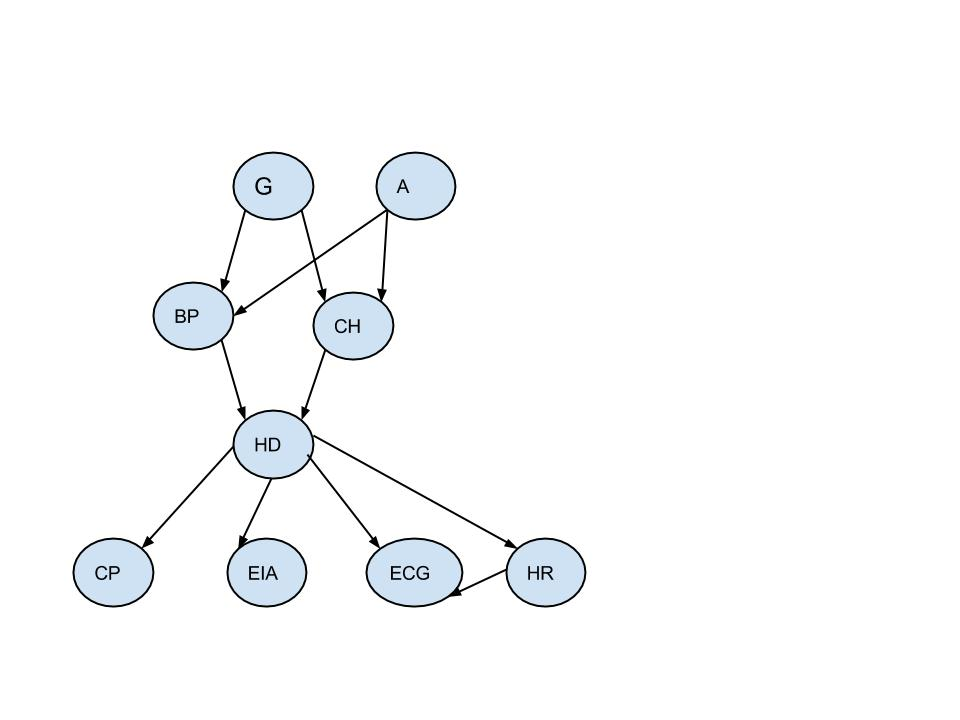
\includegraphics[scale=0.5]{BayesNet.jpg} \\
\subsection*{(b)} Factorization for above Bayes Net can be written as follows:
\begin{align*}
P(A,G,BP,CH,HD,CP,EIA,ECG,HR) &= P(A)P(G)P(BP|G, A)P(CH|G, A)P(HD|BP, CH)P(HR|HD)\\
							  & P(CP|HD)P(EIA|HD)P(ECG|HD, HR)
\end{align*}
\subsection*{(c)} Some of the choices that went into desiging network structure:
\begin{itemize}
\item I removed some irrelevant factors like dependence relationship between Age (A) and HeartRate (HR). 
\item Adding new factor or relationship between Age (A) and Blood Pressure (BP), Electrocardiograph (ECG) and Heart Rate (HR). It affect causal relationships between variables.
\end{itemize}
Hence overall the network is simplified as compared to the original given network.
\subsection*{(d)}
\begin{tabular}{|c|c|c|c|}\hline
Fold & Correct & Total & $Accuracy(\%)$  \\ \hline
1 & 44 & 60 & 73.33 \\ \hline
2 & 49 & 60 & 81.66 \\ \hline
3 & 40 & 60 & 66.66 \\ \hline
4 & 48 & 60 & 80 \\ \hline
5 & 48 & 60 & 80 \\ \hline
Mean & 45.8 & 60 & 76.33 \\\hline
\end{tabular}
\\ \\
Mean Prediction accuracy over the five test files $=76.33$. \\
Standard deviation of the prediction accuracy over the five test files $=5.61$. \\ \\
Accuracy of above designed network is better than the original network. We removed irrelevant relationships between variables and introduced new causal relationship. \\
\end{document}
